\chapter{Introduction}
\label{cha:intro}

It is astonishing how, based on the same genetic information coded into the DNA, cells in an organism can differentiate into a variety of specialized types with a multitude of different tasks.
Beginning with a single cell, a temporal, spatial and functional coordination determines the growth and body formation of eukaryotic organisms.
Depending on the cell state, only a fraction of genes is actively transcribed, while others remain repressed.
Acting as an additional regulatory layer, the epigenome describes a set of chemical modifications made to the DNA, controlling, inter alia, the activation and transcription of genes into RNA and ultimately proteins.
Present sequencing technologies and connected bioinformatics provide researchers with the tools to study sequence and epigenetic state down to single cell and single molecule resolution.
Starting 1990 and taking over a decade until completion, the human genome project incorporated an international team of researchers with the aim of deciphering for the first time the genetic blueprint to build a human being. Based on elementary sequencing technology, the outcome was already a nearly complete reference sequence including gene annotations.
Since then, the development of high-throughput sequencing technologies enabled studies of countless organisms, cell types and disease conditions. 
While being very reliable in terms of throughput and accuracy, sequenced fragments of at most few hundreds nucleotides in length still limit the readout from repetitive regions or resolution of long distance dependencies on a single molecule.




\section{Motivation}
\label{sec:intro:motivation}

Most recently, a third-generation of sequencing techniques is introducing new perspectives to the field of genome analysis by generating previously unattainable read lengths with averages in the tens of thousands of nucleotides. 
Still under active development and with frequent improvements, long-read nanopore sequencing provides new opportunities by, visually speaking, increasing the size of the puzzle pieces.
Modern nanopore sequencing devices, producing large data sets within few days, open therefore a new field of research at the intersection of genomics, computer science and engineering. 
New data types, formats and error characteristics demand here the adaptation of existing and development of new algorithms for bioinformatic software.




\section{Genome Regulation}
\label{sec:intro:bio}



\begin{figure}[h]
	\centering
	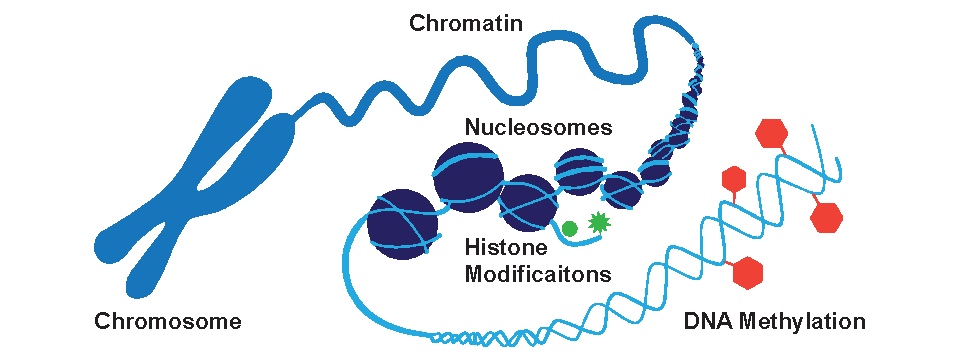
\includegraphics[width=1.0\textwidth]{figures/intro/chromatin.pdf}
	\captionsetup{format=plain}
	\caption[Structure]{Chromosome to nucleotide structure (Adapted from \cite{zymo2020})}
	\label{fig:intro:chromatin}
\end{figure}

\begin{figure}[h]
	\centering
	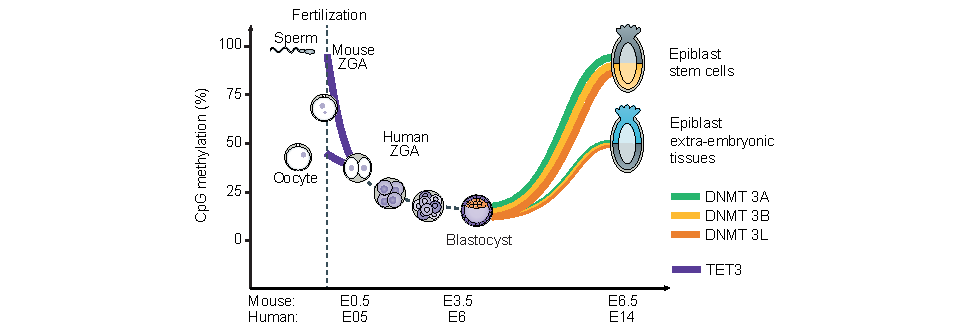
\includegraphics[width=1.0\textwidth]{figures/intro/methylation.pdf}
	\captionsetup{format=plain}
	\caption[DNA methylation dynamics]{Methylation dynamics during development (Adapted from \cite{Greenberg2019})}
	\label{fig:intro:methylation}
\end{figure}

\begin{itemize}
    \item Organism, cell, DNA
    \item Epigenetics as additional layer
    \begin{itemize}
        \item Briefly histone modifications
        \item DNA methylation, 5mC, hmC, 6mA
    \end{itemize}
    \item Without explicit statement: Focus of the Meissner lab
\end{itemize}




\section{Sequencing Technologies}
\label{sec:intro:sequencing}

\begin{figure}[h]
	\centering
	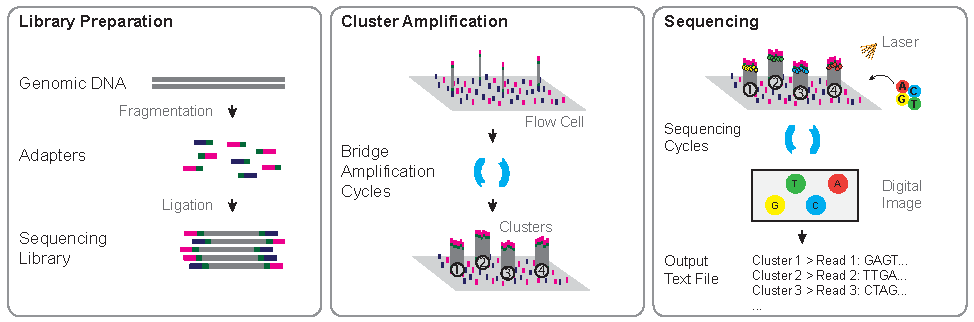
\includegraphics[width=1.0\textwidth]{figures/intro/sbs.pdf}
	\captionsetup{format=plain}
	\caption[Sequencing by synthesis]{Sequencing by synthesis}
	\label{fig:intro:sbs}
\end{figure}

\begin{figure}[h]
	\centering
	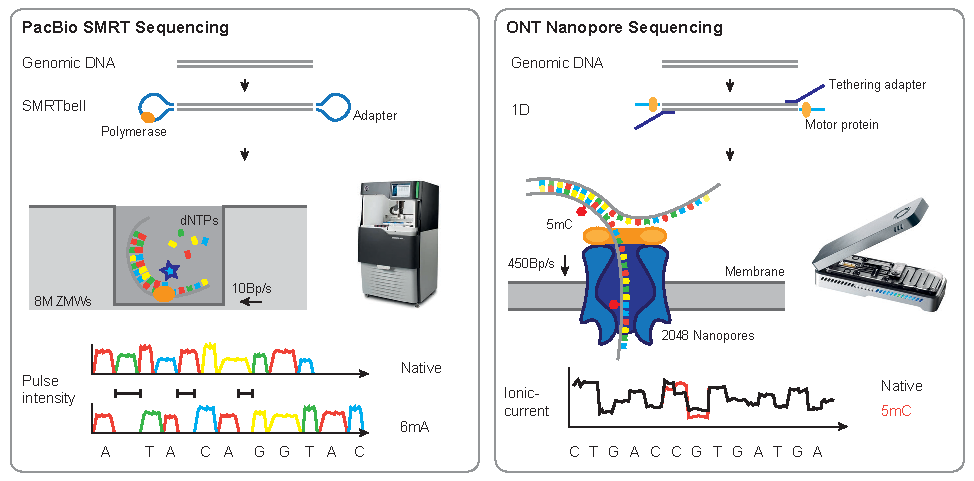
\includegraphics[width=1.0\textwidth]{figures/intro/long_read.pdf}
	\captionsetup{format=plain}
	\caption[Long read sequencing]{PacBio SMRT and ONT nanopore sequencing.}
	\label{fig:intro:longread}
\end{figure}

\begin{itemize}
    \item Sequencing
    \item Helene: "Easy to forget: but how to calculate a methylation rate from multiple reads and why minimum coverage. There is even a ref for 10X."
    \item Breifly generations, 1st, 2nd, 3rd ...
    \item Detail 3rd generation
    \begin{itemize}
        \item Briefly PacBio, Roche
        \item Detail ONT
    \end{itemize}
\end{itemize}

Among other devices distributed by Oxford Nanopore Technologies (ONT), the MinION in particular is gaining prominence. In brief, the nanopore sequencing process is based on guiding a nucleotide polymer through a pore inserted in a membrane while measuring a change in ionic current as a proxy signal over time. This signal is then interpreted to determine the underlying DNA or RNA sequence. The nanopore technology enables direct readout of sequences from individual DNA or RNA molecules, including base modifications, since no synthesis or amplification is required.




\section{Structure}
\label{sec:intro:structure}

Briefly describe the overall structure of the thesis, from literature to pipeline, signal processing and finally repeat detection.

%\textbf{Chapter \ref{sec:nanopype}} \\[0.2em]
%\blindtext

